\section*{UC11 - Generazione di un progetto}
\begin{figure}[H]
    \centering
    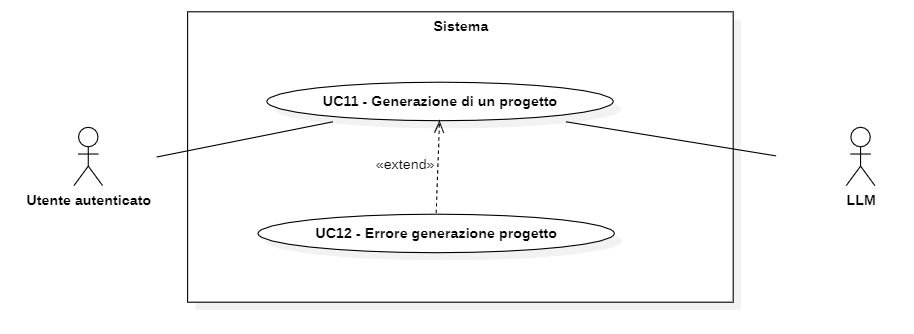
\includegraphics[scale=0.6]{usecase/uc11.png}
    \caption{UC11 - Generazione di un progetto}
    \label{fig:uc11}
\end{figure}
\begin{itemize}
    \item \textbf{Attori}: Utente autenticato, \gls{llm};
    \item \textbf{Descrizione}: L'utente avvia la generazione di un progetto utilizzando un \textit{preset};
    \item \textbf{Precondizioni}: 
    \begin{itemize}
        \item L'utente è autenticato;
        \item L'utente si trova nella pagina di creazione di un progetto ed ha selezionato un \textit{preset}.
    \end{itemize}
    \item \textbf{Postcondizioni}: Il progetto viene generato e l'utente vede le informazioni generate;
    \item \textbf{Flusso principale}:
    \begin{enumerate}
        \item L'utente compila nella sua interezza il \textit{preset} selezionato;
        \item L'utente richiede la generazione del progetto;
        \item Il sistema invia la richiesta al \gls{llm};
        \item Il \gls{llm} elabora la richiesta e genera il progetto;
        \item L'utente viene reindirizzato alla pagina di visualizzazione del progetto.
    \end{enumerate}
    \item \textbf{Estensioni}: UC12 - Visualizzazione errore generazione progetto
\end{itemize}


\vspace{0.5cm}  
\section*{UC13 - Rigenerazione completa di un progetto}
\begin{figure}[H]
    \centering
    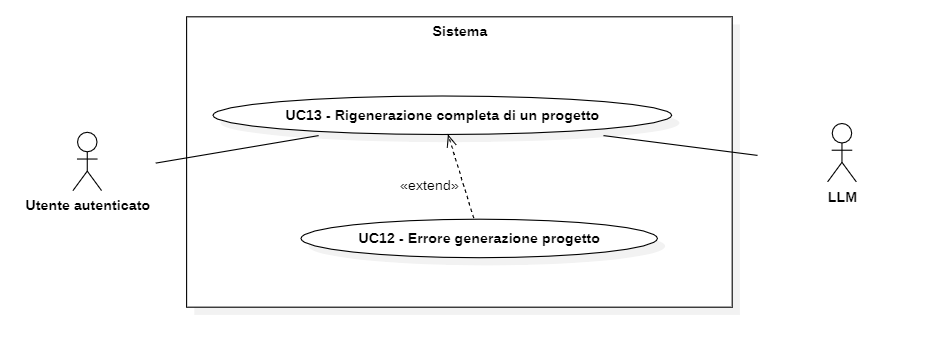
\includegraphics[scale=0.6]{usecase/uc13.png}
    \caption{UC13 - Rigenerazione completa di un progetto}
    \label{fig:uc13}
\end{figure}
\begin{itemize}
    \item \textbf{Attori}: Utente autenticato, \gls{llm};
    \item \textbf{Descrizione}: L'utente rigenera un intero progetto, sostituendo completamente il contenuto esistente;
    \item \textbf{Precondizioni}: 
    \begin{itemize}
        \item L'utente è autenticato;
        \item L'utente si trova nella pagina di visualizzazione del singolo progetto.
    \end{itemize}
    \item \textbf{Postcondizioni}: Il progetto viene completamente rigenerato;
    \item \textbf{Flusso principale}:
    \begin{enumerate}
        \item L'utente seleziona il pulsante di rigenerazione completa del progetto;
        \item Il sistema richiede all'utente l'inserimento di un \gls{prompt} su cui si baserà la rigenerazione;
        \item L'utente richiede la rigenerazione del progetto;
        \item Il sistema invia la richiesta di rigenerazione al \gls{llm};
        \item Il \gls{llm} rigenera completamente il progetto;
        \item Il progetto rigenerato viene visualizzato all'utente.
    \end{enumerate}
    \item \textbf{Estensioni}: UC12 - Visualizzazione errore generazione progetto
\end{itemize}

\pagebreak
\vspace{0.5cm}  
\section*{UC17 - \textit{Download} del progetto in formato PDF}
\begin{itemize}
    \item \textbf{Attori}: Utente autenticato;
    \item \textbf{Descrizione}: L'utente scarica il progetto in formato PDF;
    \item \textbf{Precondizioni}: L’utente si trova nella pagina di visualizzazione del singolo progetto ed ha selezionato il pulsante di visualizzazione del PDF;
    \item \textbf{Postcondizioni}: Il progetto in formato PDF viene scaricato nel dispositivo dell'utente;
    \item \textbf{Flusso principale}:
    \begin{enumerate}
        \item L’utente seleziona il pulsante di \textit{download} del progetto in formato PDF;
        \item L'utente scarica il progetto in formato PDF.
    \end{enumerate}
\end{itemize}

\vspace{0.5cm}  
